
\documentclass[a4paper,12pt,single,pdftex]{scrartcl}
\usepackage{ngerman}
 \usepackage{color}  
 \usepackage{html}  
 \usepackage{times}  
 \usepackage{graphicx} 
 \usepackage{fancyheadings}  
 \usepackage{hyperref}  
 \setlength{\parindent}{0.6pt} 
 \setlength{\parskip}{0.6pt} 
 \title{Draft}
 

\begin{document} 
\maketitle
\newpage

\label{ID_492861276}\label{ID_1956039038}\section{引言}

\label{ID_1883815321}\subsection{研究意义}

\label{ID_84459052}\subsubsection{众所周知地震灾害是关系到国计民生的重大自然灾害,虽然极具破坏的大地震发生频率很低,但是一次地震所爆发的能量却是与吨级核爆相当\citep{Stein2003},其破坏性不言而喻。2008年5月12号的汶川地震是自唐山地震以来在我国发生的导致直接死亡人数最多,经济损失最大的重大地震。然而,另一方面,地震的高能量所激发的高穿透力的地震波却是地震学家研究地球结构的福音,是人类目前研究地球内部结构的最有力工具。所以,无论从人民生活安全,经济保障,还是从科学探索的角度看,地震学研究都是很有意义的。}

\label{ID_219947997}\subsubsection{地震学研究的主要内容包括震源以及地下结构研究,震源机制是震源最基本的参数,其结果可进一步应用于理论震动图计算\citep{Wald2005}、海啸模拟\citep{Satake2007}、库仑应力转移估计\citep{King2007}、区域的应力分析和震源破裂过程反演中\citep{Kilb2001}。此外,利用已知震源机制计算得到面波震动图,用于在介质结构研究中代替到时或面波频散数据,以获得更多约束信息,直接拟合实际波形反演地下结构的方法也得到了广泛应用\citep{Nolet1990,Manaman2011,Friederich2003,Zielhuis1994,Cao2001,Lee1997}。因而在地震发生后,获得可靠的震源机制是有益且必要的。}

\label{ID_1359524240}\subsubsection{由于真实情况下,通常获得的观测数据质量都不是完美的,为了得到更为准确和可靠的震源机制,震要在反演过程中尽可能优化结果。理论上,在给定观测数据和目标函数情况下,对于结果的最大调控来自于反演的权重。合理的权重能使得对现有数据中有用信息更充分的应用,而压制无效噪声对反演的干扰影响。不同的加权得到的结果往往有差异,为了反演得到可靠的震源机制,必须谨慎考虑,合理地为数据加权。
另一方面,因为数据中的噪声具有随机性,使得反演结果相对真值有不可准确预料的偏差。事实上,反演结果与真实值的偏差还来源于参考模型的系统误差,数值计算舍入误差,理论的近似引起的偏差等等。在此仅关注研究数据噪声引起的误差,为了方便,本文之后所提的误差除非特别指出,否则均指数据随机噪声导致的震源机制误差。正是因为误差不可预料,为了使结果具有科学参考价值,必须对噪声可能导致的误差范围进行评估。排除数据噪声影响的“理想“结果则包含在反演结果的误差范围内。虽然无法直接求出该“理想”结果,但至少能在一定置信区间内给出可靠的结果范围,对于借鉴以及进一步深入研究均具有重要意义。此外,对于某些算法而言(如本文反演所用的格点搜索算法),无论结果是否可信反演后均会得到一个“最优解”,但当涉及病态反演问题时,该震源机制很可能与真实情况有非常大偏差,未经过误差评定,结果可能对之后研究者具有误导作用。}

\label{ID_1577841117}\subsection{研究发展历程}

\label{ID_459272874}\subsubsection{方法分类}

\label{ID_851024883}\paragraph{利用地震波信息反演震源机制根据反演数据源差异主要可以分为三大类方法。第一类是P波极性反演,利用了初至波第一次起跳方向信息约束震源,但对台站分布要求高,且结果不太稳定;第二类是用振幅定量信息反演,利用各震相的振幅的差异或方位特性等定量信息进行反演,但续至波的振幅观测通常比较困难;第三类是波形拟合反演,直接利用整个波形数据的所有可用信息计算震源机制,对相对约束效果更好。}

\label{ID_894502911}\subsubsection{P波初动极性反演}

\label{ID_1137644143}\paragraph{早期的震源机制反演根据P波初动极性在四象限中的分布规律\citep{Balakina1961},这首先起源于\citep{Reid1910}在1906年旧金山地震研究\citep{Milne1910}基础上提出了弹性回跳理论——认为地震是由于地壳中岩石积累了过多应变能,超过其承受能力后,发生弹性断裂,势力随之释放。之后,P波初动符号的规律被发现\cite{Nakano1923},人们提出了地震节面的概念。后来便开始利用地震台站记录到的地震波初动极性信息在被地震节面分隔的四象限空间的分布,对震源节面进行约束,进而得到震源机制。然而由于该方法仅使用了初动极性这一少量信息,并且初动极性的明显性与初动P波振幅相关,理论上在四象限节面上P波振幅为0\citep{Stein2003}。以上种种原因导致该方法适用性受限,且结果不太稳定,为了得到稳定结果该方法对台站数据的数量和分布要求很苛刻。}

\label{ID_1069715761}\subsubsection{振幅比反演}

\label{ID_1788012684}\paragraph{第二类方法是利用各震相的振幅的信息,这是使用波形振幅数值的定量信息,增加反演数据的可用约束信息。例如利用P,S波的振幅比信息,通过同一台站不同分量震相信息比值规律,可一定程度避免来自介质模型不准确的系统性误差影响。其中利用P震相与SV震相的震幅比\citep{Kisslinger1982,Kisslinger1980}是一种行之有效的方案,为了最大程度削弱介质模型对反演的影响,选择了直达上行地球表面的Z分量波。此外,在Kisslinger研究基础上,发现当有较高质量SH波时,通过P震相与SH震相的振幅比值反演可能得到更可靠的震源机制。另外,也有利用面波的振幅花样\citep{Stein2003}反演震源机制等可行方案。虽然利用振幅信息有效增强了对震源的约束,但是仍然对台站分布有较高要求,而且对近震波形S波初至振幅的测量,尤其是SV波的测量显得尤其困难\citep{祁玉萍2013},稍有不慎便可能得到较大偏差。}

\label{ID_1555876496}\subsubsection{波形拟合反演}

\label{ID_1741964446}\paragraph{波形拟合反演直接利用了整个波形数据的所有信息进行反演,随着理论地震波的研究取得巨大成功\citep{Haskell1964,Herrmann1979,Wang1980},在给定介质模型和震源机制情况下可以比较精确地计算出理论波形,使得直接使用观测波形数据与理论数据匹配反演震源机制的想法得以实现。通常波形中的体波数据由于穿透深,受浅层不均匀地壳结构影响较小,但考虑到体波衰减快,通常利用远震体波反演较大地震的震源机制,这能够减小地下介质模型横向非均匀性影响。而面波对介质结构较敏感,则较常用于具有较为精确介质参考模型的区域地震震源研究,或结合震源机制研究其较为敏感的地下结构\citep{Nolet1990}。由于波形数据相比初动极性或振幅,包含了更多有效信息,使得对台站数量及分布的要求有所降低,且结果更稳定,可靠,于是波形拟合反演的方法得到了快速发展和应用\citep{Walter1993,Ritsema1993,Zhao1994,Nabvelek1995}。}

\label{ID_1436540560}\paragraph{用地震波形拟合反演震源机制时,由于待求参数少、解空间有限且观测方程直接求解异常复杂,所以该问题非常适合用非线性反演中的全局搜索算法。在实践中,得到广泛应用的CAP(Cut and Paste的简称)\citep{Zhao1994,Zhu1996,Tan2006}和CPS(Computer Programs in Seismology的简称)\citep{Herrmann1989}等波形拟合反演程序充分说明了全局搜索在震源机制反演问题中的有效性。}

\label{ID_1102145719}\subsection{波形反演现状及问题}

\label{ID_138447139}\subsubsection{Herrmann开发的CPS软件包中用于震源机制反演子程序的方法\citep{Herrmann1989}(为方便本文简称CPS方法)和CAP方法\citep{Zhao1994,Zhu1996,Tan2006}均为震源机制格点搜索方法,由于二者的实用性和开源性,被广泛应用于震源机制研究中。然而CAP和CPS方法加权的侧重点不同,前者考虑几何扩散导致波形振幅的衰减,给较低振幅的波形加大权重,以平衡不同振幅波形在反演中的影响力;后者则关注传播过程中信噪比的降低,赋予高信噪比数据较大权重。考虑到波形振幅及信噪比与震中距间的关系,Zhu等\citep{Zhu1996}在CAP中将权重设置为关于震中距递增的幂函数,而CPS方法中使用震中距的反比例函数作为权重值。幂函数和反比例函数的单调性恰巧相反,导致从数值上看,两种方法对同一套数据波形所定权重大小相互矛盾——CPS定权震中距较近台站权重较高,而CAP定权中则震中距较远台站相对权重较大。此外,通过实例计算及理论分析发现,实际观测波形的振幅及信噪比与震中距的关系较为复杂,难以用简单的初等函数进行描述,且函数中包含的参数赋值因人而异。因此无论利用幂函数或反比例函数估算的振幅和信噪比均较粗糙,无法准确体现数据的真实性和客观性。}

\label{ID_1797636015}\subsubsection{另一方面,随着CAP,CPS等用波形非线性反演震源机制的算法得到广泛应用\citep{Luo2015,D’Amico2014,赵博2013},其非线性反演中误差缺失的问题逐渐受到了关注。考虑到误差评价的重要性,国内外学者均对震源机制反演的误差估计问题进行了研究,Duputel等\citep{Duputel2012}从误差的来源入手,对震源机制进行误差评价,但其方法只适用于估计线性反演的震源机制误差。考虑到目前应用最广泛的全局搜索反演,本文旨在探究能应用于非性线反演算法的误差评估方法。对于非线性反演,最常见的方法是对目标函数的极值人为给定一个阈值,满足该条件的所有解构成误差范围内解集(简称为阈值法),该方法简洁直观,能快速发现不同模型参数的误差大小关系,但是阈值的给定有主观性,导致定量结果难以让人信服。郑建常等\citep{郑建常2015}借鉴Bootstrap(Efron1979)的思想,对数据集随机多次选取子集进行独立反演并对解集样本用一定方法分析,以评估其整体误差及解,为使样本能反映整体。但是统计分析不仅要求样本抽取的随机性,还对原始样本大小有一定要求,当可用的地震记录数量不是很大时基于重抽样的该方法便不适用了。}

\label{ID_616390154}\subsection{本文设定目标及方案}

\label{ID_1218200436}\subsubsection{针对以上分析,为了解决CPS和CAP反演定权方法出现的矛盾以及误差缺失问题,本文分别尝试进行权重优化以及误差评定。对于定权,结合CPS与CAP,综合考虑振幅衰减和信噪比差异影响,将二者统一计算权重,从而解决上述的权重数值矛盾问题。其次,计算时摈弃了用震中距简单函数估算振幅或信噪比方案,而是基于每道波形数据自身的信息,准确评估振幅和噪声。由于没有人工干预,在提高精确度的同时有效保证了客观性。}

\label{ID_1099326584}\subsubsection{为了解决反演震源机制时误差估计的问题,本文借鉴了\citet{Hardebeck2002}对P波初动极性反演方法改进的思路——首先估计观测数据的随机误差大小,据此模拟随机误差,并将其加入原始数据生成多组模拟数据集,最终反演得到一系列误差范围内的解集。该方法不仅估计了误差,且使得反演结果更稳定\citep{Hardebeck2002}。将该思想应用到波形反演震源机制的问题中,利用评估噪声随机模拟多套波形数据集,并用每套数据分别进行反演,得到包含多次反演结果的解集,并对解集统计分析得到解的误差(为方便叙述称其为模拟分析法)。本文方法与重采样类方法\citep{郑建常2015,Efron1979}不同的是每次反演的数据并非原始数据集的子集,而是与数据集等价的模拟数据集,保留了原数据集的样本大小,更重要的是每套数据均具有一致的数据分布结构。所以对观测数据的数量要求相对降低,能比重采样类方法更好应用于台站记录较稀少的地震事件。}

\label{ID_323720947}\subsubsection{为了验证本文提出权重优化方案和误差评价方法的有效性,基于CPS反演程序进行了一系列理论试验,分别检验权重优化效果和误差估计与理论预测是否吻合。对同一个设定条件下的模拟地震进行了三次试验,分别测试误差评价时重复反演次数的设定值,误差评定方法对噪声的反应情况,权重优化的效果。第一次试验研究误差评价时反演的重复次数对最终结果的影响,用以为该方法在应用时选择合适的反演次数。试验分别尝试了重复20次,40次,60次,80次和100次,结果发现该方案对反演次数不是特别敏感,结果基本一致且可信。为保证样本量充足,选定100次为默认反演次数。第二次试验测试结果误差对数据噪声的反应是否合理,对理论事件加噪时分别加了低,中,高,超高强度噪声,反演结果确实体现了误差由低到高的趋势,而且理论真值均在误差范围内,表明了本文误差估计的真实性和稳定性。第三次试验则分别设定了单独信噪比加权,单独振幅调节加权,信噪比和振幅调节联合定权三组对照组。三组对照组反演结果均在误差范围内包含真值,但是综合看来联合定权的平均误差是最小的,体现了联合定权的优越性。}

\label{ID_1381199343}\subsubsection{为了体现本文方法的实际应用性,以2013年4月20日的芦山地震为例,分别采取单独振幅调节加权、单独信噪比加权以及振幅调节和信噪比调节联合加权的策略进行三次反演,并利用本文的误差估计方法对三次反演的结果进行评价。通过对结果的合理性及平均误差两方面进行讨论,以真实案例证实本文联合加权策略反演结果最优,对应的震源机制解为(走向200°,倾角38°,滑动角89°),震源深度18km,与其它研究者的研究成果有很好的一致性,且与震源区的应力及地质构造情况均相互吻合。}

\label{ID_64212303}\section{原理分析}

\label{ID_67382634}\subsection{震源基础概念}

\label{ID_72470361}\subsubsection{1906年旧金山发生了一次在地震学上具有重在研究意义的地震,地震前后对圣安德烈亚斯断层的研究结果\citep{Milne1910}使人们普遍认为发生地震的原因是震源处的断层发生了滑移错动,巨大的势能转化为了热能及地震波等能力。这种错动可由位错理论进行解释,位错理论认为地震的发生是因为应力长期缓慢的大量积累,最终达到了断层锁定的极限,引发断层面(原有断层或地震新生断层)两侧发生突然的位错,导致了应力释放并形成地震。自此以后,对于地震震源的研究就开始集中到断层面的研究上。通常认为断层面两侧的应力在地震发生前后都是连续的,只有位移在断层面两侧突然间断,所以研究清楚断层面上的所有运动学信息是研究整个震源过程的主要内容。如果进一步简化,将地震发生时断层的位错视为纯剪切的点源位错(事实证明该简化很多情况下是合理的,且本文只讨论该情况),则利用三个描述断层的参数便可完整描述震源的物理过程(不考虑时间函数),并称该三参数为震源的机制解。求解震源机制的过程便是求解该三个参数的过程,该三参数具体定义如图\ref{fig01}所示\citep{程万正2006}。
\begin{figure}
\centering
  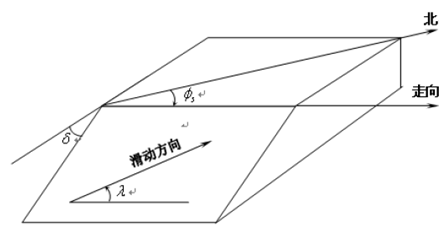
\includegraphics{fig01.png}
  \caption{震源机制三个参数的具体意义}
  \label{fig01}
\end{figure}}

\label{ID_1219588045}\subsection{波形拟合反演}

\label{ID_1243921566}\subsubsection{波形分解}

\label{ID_1903486780}\paragraph{}

\label{ID_1523655541}\paragraph{其中 $s(t)$为震源时间函数,$Mkj$为地震矩张量,$G_{nk,i}$为格林函数,从上式可知理论波形$d$与$Mi$为线性关系。根据\citet{Kikuchi1991}的分解方法,任意地震矩张量均可由6个简单地震矩张量通过线性组合而成,如公式\ref{eq02}。
\begin{equation}
\label{eq02}
M=\sum_{k=1}^6a_kM_k
\end{equation}}

\label{ID_1003994788}\paragraph{公式\ref{eq02}中等式右边的$M_k$如公式\ref{eq03}所示。
\begin{equation}
\label{eq03}
\begin{array}{ccc}
M_1=\left[\begin{array}{ccc}
0 &amp; 1 &amp; 0\\
1 &amp; 0 &amp; 0\\
0 &amp; 0 &amp; 0\\
\end{array}\right],&amp;
M_2=\left[\begin{array}{ccc}
1 &amp; 0 &amp; 0\\
0 &amp; -1 &amp; 0\\
0 &amp; 0 &amp; 0\\
\end{array}\right],&amp;
M_3=\left[\begin{array}{ccc}
0 &amp; 0 &amp; 0\\
0 &amp; 0 &amp; 1\\
0 &amp; 1 &amp; 0\\
\end{array}\right],\\
M_4=\left[\begin{array}{ccc}
0 &amp; 0 &amp; 1\\
0 &amp; 0 &amp; 0\\
1 &amp; 0 &amp; 0\\
\end{array}\right],&amp;
M_5=\left[\begin{array}{ccc}
-1 &amp; 0 &amp; 0\\
0 &amp; 0 &amp; 0\\
0 &amp; 0 &amp; 1\\
\end{array}\right],&amp;
M_6=\left[\begin{array}{ccc}
1 &amp; 0 &amp; 0\\
0 &amp; 1 &amp; 0\\
0 &amp; 0 &amp; 1\\
\end{array}\right],\\
end{array}
\end{equation}}

\label{ID_1895578740}\paragraph{$M_1$-$M_6$为6个简单的地震源,其中$M_6$代表爆炸源,其余5个均为剪切位错源,根据公式\ref{eq02}和公式\ref{eq03}推导可知系数a与M各分量间的对应关系如公式\ref{eq04}和公式\ref{eq05}。
\begin{equation}
\label{eq04}
M=\left[\begin{array}{ccc}
a_2-a_5+a_6 &amp; a_1 &amp; a_4\\
a_1 &amp; -a_2+a_6 &amp; a_3\\
a_4 &amp; a_3 &amp; a_5+a_6\\
\end{array}\right]\\
\end{equation}

\begin{equation}
\label{eq05}
\left[\begin{array}{c}
a_1\\
a_2\\
a_3\\
a_4\\
a_5\\
a_6\\
\end{array}\right]=
\left[\begin{array}{c}
M_{12}\\
(M_{11}+M_{33}-2M_{22})/3\\
M_{23}\\
M_{13}\\
(2M_{33}-M_{11}-M_{22})/3\\
(M_{11}+M_{22}+M_{33})/3\\
\end{array}\right]
\end{equation}}

\label{ID_733899755}\paragraph{将公式\ref{eq02}代入公式\ref{eq01},并省略波形分量指标$n$可得到公式\ref{eq06}。
\begin{equation}
\label{eq06}
d=\sum_{k=1}^{6}a_kd_k
\end{equation}}

\label{ID_362828610}\paragraph{再将公式\ref{eq05}所示的$a$与$M$关系代入公式\ref{eq06}可得到$d$关于$M$与$d_k$的公式\ref{eq07}。
\begin{equation}
\label{eq07}
\begin{array}{l}\\
d=&amp;M_{11}(1/3d_2-1/3d_5+1/3d_6)+M_{12}d_1+M_{13}d_4\\
&amp;+M_{22}(-2/3d_2-1/3d_5+1/3d_6)+M_{23}d_3\\
&amp;+M_{33}(1/3d_2+2/3d_5+1/3d_6))
\end{array}
\end{equation}}

\label{ID_1164082214}\paragraph{为进一步简化,将公式\ref{eq07}中$M$矩阵的6个分量依次记为 $M_1,M_2,M_3,M_4,M_5,M_6$,并将与$Mi$相乘的关于$d_k$的多项式简记为$G_i$,于是得到了简洁的6项求和的理论波形公式\ref{eq08}。在此我们按照\citet{Stein2003}专著中关于地震矩反演章节中对格林函数的推广定义,将公式\ref{eq08}中的$G_i$也称为格林函数,此格林函数即是我们之后在CPS反演中需要用到的。
\begin{equation}
\label{eq08}
d=G_iM_i(i=1,2,...6)
\end{equation}}

\label{ID_1125175989}\paragraph{于是任意地震矩产生的波形均可由其矩张量矩阵和6个格林函数线性叠加得到,而格林函数又可由6个已知基本地震矩激发的波形$d_k(k=1,2,...6)$叠加得到。由于以上运算均是线性运算,在$d_k$已知的情况下,在计算机中经两次迭加得到$d$速度非常快。}

\label{ID_1890175740}\paragraph{至此,我们已经将任意剪切位错源的波形分解为6个基本震源波形的线性叠加,而叠加的系数可由该位错源的震源机制唯一确定。现在的关键问题转化为计算6个基本震源对应的理论波形$d_k$,这可通过之后要介绍的格林函数库快速实现。}

\label{ID_1740220633}\subsubsection{格林函数库}

\label{ID_100364337}\paragraph{通常情况下天然地震由断层间错动造成,震源均近似纯剪切位错源。习惯上人们用破裂断层的三个角度参数——走向,倾角和滑动角来更直观地描述震源机制,地震矩张量与震源机制三个参数的对应关系如公式\ref{eq09}所示\citep{Aki1980}。
\begin{equation}
\label{eq09}
\left\{
    \begin{array}{l}
    M_{11}=-M_0(sin{\delta}cos{\lambda}sin{2\phi_s}+sin{2\delta}sin{\lambda}sin^2{\phi_s})\\
    M_{12}=M_0(sin{\delta}cos{\lambda}cos{2\phi_s}+1/2sin{2\delta}sin{\lambda}sin{2\phi_s})\\
    M_{13}=-M_0(cos{\delta}cos{\lambda}cos{\phi_s}+cos{2\delta}sin{\lambda}sin{\phi_s})\\
    M_{22}=M_0(sin{\delta}cos{\lambda}cos{2\phi_s}-sin{2\delta}sin{\lambda}cos^2{\phi_s})\\
    M_{23}=-M_0(cos{\delta}cos{\lambda}sin{\phi_s}-cos{2\delta}sin{\lambda}cos^2{\phi_s})\\
    M_{33}=M_0sin{2\delta}sin{\lambda}\\
    \end{array}
\right.
\end{equation}}

\label{ID_650574393}\paragraph{其中,$\phi_s$是走向,$\delta$是倾角,$lambda$是滑动角。 $M_0$是最早由\citet{Aki1966}提出的用来度量震源长周期辐射的强度,最初称为地震矩。由于是一个标量,现在又叫作标量地震矩,代表了地震的强度。将公式\ref{eq09}代入公式\ref{eq08}即将公式转化为了理论波形关于震源机制三参数的形式。}

\label{ID_1121124158}\paragraph{现在我们进一步研究$d_k$如何计算,在均匀介质\citep{Ben-Menahem1963}和层状介质\citep{Haskell1964}模型的面波波场辐射理论基础上,\citet{Wang1980} 进一步得到了剪切位错源在层状速度模型中所激发的地震波场,在柱坐标频域下的表示,如公式\ref{eq10}所示。
\begin{equation}
\label{eq10}
\left\{
    \begin{array}{l}
    U_z(r,\phi,0,\omega)=Z_{SS}{\cdot}s_2+Z_{DS}{\cdot}s_3+Z_{DD}{\cdot}s_1\\
    U_r(r,\phi,0,\omega)=R_{SS}{\cdot}s_2+R_{DS}{\cdot}s_3+R_{DD}{\cdot}s_1\\
    U_{\phi}(r,\phi,0,\omega)=T_{SS}{\cdot}t_2+T_{DS}{\cdot}t_1\\
    \end{array}
\right.
\end{equation}}

\label{ID_1825707031}\paragraph{公式\ref{eq10}中各符号意义如\ref{eq11}所示,\ref{eq11}中$\phi$是地震观测台站相对震源的方位角,$\lambda$,$\delta$,${\phi}_s$分别代表断层滑动角,倾角,走向。公式\ref{eq10}中的$Z_{SS}$,$R_{SS}$,$T_{SS}$分别对应于$\delta=90^\circ$,$\lambda=0^\circ$的纯走滑型断裂的理论地震图的垂向、径向、切向分量;$Z_{DS}$,$R_{DS}$,$T_{DS}$分别代表$lambda=90^\circ$,$\delta=90^\circ$的纯倾滑型逆冲断层激发的地震波的垂向、径向、切向分量;$Z_{DD}$和$R_{DD}$分别对应于倾角$\delta=45^\circ$,滑动角$\lambda=90^\circ$的逆冲断层激发的理论地震波的垂向、径向分量。它们8个是合成任意剪切位错源理论地震图所需要的全部基本函数,它们是对波数K的积分表达\citep{Wang1980} 。格林函数库即由大量的不同震中距,不同震源深度对应的这8个基本函数组成。
\begin{equation}
\label{eq11}
\left\{
    \begin{array}{l}
    s_1=1/2{sin\lambda}sin{2\delta}\\
    s_2={cos\lambda}{sin\delta}sin2({\phi}-{\phi}_s)+1/2{sin\lambda}{sin2\delta}cos2({\phi}-{\phi}_s)\\
    s_3=-{cos\lambda}{cos\delta}cos({\phi}-{\phi}_s)+{sin\lambda}{cos2\delta}sin({\phi}-{\phi}_s)\\
    t_1={cos\lambda}{cos\delta}sin({\phi}-{\phi}_s)+{sin\lambda}{cos2\delta}cos({\phi}-{\phi}_s)\\
    t_2={cos\lambda}{sin\delta}cos2({\phi}-{\phi}_s)-1/2{sin\lambda}{sin2\delta}sin2({\phi}-{\phi}_s)\\
    \end{array}
\right.
\end{equation}}

\label{ID_1685002795}\paragraph{利用公式\ref{eq09}可推算出公式\ref{eq03}中所示6个基本地震所对应的震源机制,即各地震的3个角度参数,将其代入公式\ref{eq10},并积分变换到时间域,便得到了$d_k$,进而得到$d$。而根据公式\ref{eq11}知$s_1$、$s_2$、$s_3$、$t_1$、$t_2$等量均与$\omega$无关,结合公式\ref{eq10}可推得时间域的$Z_{SS}$,$R_{DD}$等量与$d_k$的关系也是线性的,可通过快速线性叠加得到。
综上分析知,计算$d$的关键在于得到该速度模型下,对应震中距和震源深度的$Z_{SS}$,$R_{DD}$等基本函数。而计算该函数由于要经过大量积分运算,计算速度非常慢,在迭代或搜索反演过程中实时计算一系列该基本函数是不可取的。在实际工作中通过将研究区域按一定精度格点划分,并事先计算好各格点的基本函数,并将大量的各点所对应的基本函数归档存储为格林函数库。之后理论波形数值计算需要时,直接在格林函数库中调用对应震中距和震源深度的基本函数即可,这样便实现了$d$的快速计算。经检验,这样叠加计算理论波形的速度非常快,能满足格点搜索时大量理论波形图计算的需要。}

\label{ID_424266573}\subsubsection{格点搜索}

\label{ID_1321964956}\paragraph{CAP与CPS方法计算波形的拟合度时使用了不同的目标函数,CAP方法先将理论波形与实测波形通过互相关运算进行时差调整,再计算调整后的波形间残差范数(L1或L2)\citep{Zhao1994},该残差范数定为为最终的目标函数,CPS方法则直接将理论与实测波形的互相关函数作为目标函数。为了单独分析权重因素对反演的影响,对比CPS与CAP不同定权的差异,后文反演试验及讨论均基于CPS的目标函数方案。CPS方法中的互相关目标函数Fit如公式\ref{eq12}定义。
\begin{equation}
\label{eq12}
Fit=(\int_{Tb}^{Te}Y(t)G(t)dt)^2/(\int_{Tb}^{Te}Y(t)Y(t)dt*\int_{Tb}^{Te}G(t)G(t)dt)
\end{equation}}

\label{ID_143427010}\paragraph{在计算机中进行数值计算时使用公式\ref{eq13}所示离散形式:
\begin{equation}
\label{eq13}
Fit=[\sum_{j=1}^{N}\sum_{m-1}^{6}yg(j,m,k)M_m]^2/{[\sum_{j=1}^{N}yy(j)][\sum_{j=1}^{N}\sum_{m=1}^{6}\sum_{n=1}^{6}gg(j,m,n)M_mM_n]}
\end{equation}}

\label{ID_247138940}\paragraph{公式\ref{eq13}中各符号表示的含义如公式\ref{eq14}和公式\ref{eq15}所示。
\begin{equation}
\label{eq14}
\left\{
    \begin{aligned}
    yy(j)&amp;=\sum_{h=1}^{H(j)}y(j,h)y(j,h)wt(j)\\
    gg(j,m,n))&amp;=\sum_{h=1}^{H(j)}g_{m}(j,h)g_{n}(j,h)wt(j)\\
    yg(j,m,k))&amp;=\sum_{h=1}^{H(j)-|k|}\mathop{{y}'}(j,h)\mathop{{g}'_{m}}(j,h)wt(j)
    \end{aligned}
\right.
\end{equation}}

\label{ID_457268259}\paragraph{\begin{equation}
\label{eq15}
\left\{
    \begin{aligned}
    \mathop{{y}'}(j,h)&amp;=y(j,h+k) &amp;k\geq0 \\
    \mathop{{g}'}(j,h)&amp;=g(j,h)   &amp;k\geq0 \\
    \mathop{{y}'}(j,h)&amp;=y(j,h)   &amp;k&lt;0 \\
    \mathop{{g}'}(j,h)&amp;=g(j,h-k) &amp;k&lt;0 \\
    \end{aligned}   \\
\right.
\end{equation}}

\label{ID_31082694}\paragraph{}

\label{ID_1372162761}\paragraph{理论地震图可用多种方法计算,本文通过之前章节所述的用格林函数库快速合成理论波形,而格林函数库则用CPS软件包中的hprep96,hspec96,hpulse96子程序计算得到,该子程序的基本原理是波数积分法。反演时考虑到震源机制解的全空间(走向0°-360°,倾角0°-90°,滑动角-180°-180°)较小,通常采用全空间格点搜索法。
格点搜索法将全空间划分为一定精度间隔的格点,并依次遍历全部格点找寻目标函数最值点,最值处对应格点即为最优解。本文如公式\ref{eq13}所示目标函数Fit的具体计算过程如下,将遍历到的格点震源机制转换为等价地震矩张量\citep{Jost1989},同时用格林函数库快速求出公式\ref{eq08}中对应的格林函数$Gi$,将格林函数$Gi$,观测波形$d$进行必要且相同的滤波、截取时窗处理,并将处理后格林函数$g$,观测波形$y$和地震矩张量$M$与代入公式\ref{eq13},计算即可求得该格点处的拟合度Fit。}

\label{ID_1583356182}\subsection{数据质量影响}

\label{ID_1185228221}\subsubsection{数据质量意义}

\label{ID_1489213091}\paragraph{一般反演的概念是指在给定观测数据情况下,选定一个反演标准,即目标函数,如误差最小二乘标准(简称最小二乘标准),模型最小二范数标准等,然后依赖待反演模型与观测数据的理论关联公式,按选定的目标函数寻找最优的模型。具体寻找最优模型的方法称为反演方法,如线性反演方法(牛顿法,共轭梯度法等),非线性反演方法(模拟退火,遗传算法,以及本文的格点搜索方法等)。然而需要明白,在理想情况下(即不考虑计算过程中产生的各种数值误差,各算法的复杂度,理论公式的近似性,结构性系统误差等),待求模型的最终结果与反演算法是无关的,而是由反演标准和输入观测数据两者唯一决定,不同反演算法差异只是体现在寻找该最优解时的效率和准确度上。

因此,当反演标准确定的情况下(例如本文反演所使用的波形互相关拟合标准),对反演结果具有决定性的就是原始的观测数据。不同的观测数据决定了不同的反演结果,良好的观测数据对应着与真值接近的反演结果。通常我们用数据质量来描述观测数据的好坏,数据质量又可分为数据信噪比和数据结构两方面。}

\label{ID_1247587863}\subsubsection{数据信噪比}

\label{ID_551492897}\paragraph{顾名思义,数据信噪比代表在观测数据中,难以分离的有用信号与无用噪声的比值,是对数据真实程度的一个评价。信噪比越差,代表该数据包含的真实有用信息越少,而随机噪声对反演结果产生的不确定性干扰也可能越大。如果噪声超过了一定极限值,真实信号完全淹没在噪声中,反演结果基本由噪声决定,完全失去了参考价值,甚至产生严重的误导作用。所以实际反演时,会采用一系列办法尽量争取高信噪比输入,以保证结果的可靠性。常用的手段如高噪声数据剔除、滤波压制噪声、合理分配权重抑制强噪声数据影响等。}

\label{ID_269467231}\subsubsection{数据结构}

\label{ID_1245351596}\paragraph{数据结构在本文中指代数据对待求模型的约束力度,同时包括数据容量和分布状况。在反演过程中体现为观测方程对待解模型参数能否确定,较差的数据结构对应着反演中的模型欠定情况。实际反演中,观测数据的数据结构越差,对待求模型的约束效果越弱,越可能出现在同一反演标准下多解的情况,并且各解在当前反演系统下等价,无法区分。在波形反演中,为了改良数据结构,可以选用方位分布良好的台站数据作为反演输入,通过合理权重配比调整各数据在反演中的影响,以对模型参数有更强约束。}

\label{ID_883941621}\subsubsection{小结}

\label{ID_1030551001}\paragraph{数据信噪比和数据结构是决定数据质量的两个相对独立的方面,单纯高信噪比并不代表好的数据质量,若数据结构太差,可能导致反演时找到一系列完美符合反演标准的解,却无法分辨其中哪个解才是真实的。相反,即使信噪比稍低,但若具有同样良好的数据结构,通过反演解算即使无法找到达到完美反演标准的解,但最优解却与其它解差别比较明显,易于保证解的唯一性。

反演时,需要同时兼顾数据质量的两方面,通过数据预处理或合理的权重配比能一定程度改善数据结构。}

\label{ID_1003053734}\subsection{定权优化方案}

\label{ID_975012270}\subsubsection{反演通常采用大量波形数据,而数据在反演中所占权重会对最终结果有决定性影响,因此合理设置$wt$值非常重要。CPS方法从数据的信噪比着手定权,考虑到信噪比随震中距增加而下降的趋势,将权重设为震中距的反比例函数,台站震中距越远的数据权重越小。CAP方法\citep{Zhu1996}则注意到波形间振幅的差异,高振幅的波形数据对反演结果起主导作用,导致低振幅波形的数据信息得不到充分利用。考虑到几何扩散是导致振幅衰减的重要原因,CAP令$wt$为震中距的幂函数,使得震中距远的台站权重相对较大,以补偿振幅的衰减。综上可知CAP和CPS方法的权重分别侧重考虑调节波形振幅和信噪比的差异。振幅调节的作用是当有振幅差异较大的多道波形参与反演时,防止强振幅的波形主导反演结果,使不同振幅的波形对反演具有相当的贡献,所以当有大量有振幅差异的波形数据参与反演时,为充分利用各道波形的信息约束反演结果必须设置振幅调节权重因子。但另一方面,振幅调节权重会进一步放大数据信噪比的差异,所以还应合理考虑信噪比定权,使高信噪比数据在反演中具有较大的影响力。基于上述分析,本文联合CPS与CAP的加权方案,将信噪比权重项$wt1$与振幅调节权重因子$wt2$的乘积设为最终的权重因子$wt$。}

\label{ID_1260250456}\paragraph{$wt$对反演具有决定性影响,CPS方法将其设为与震中距负相关的信噪比权重因子,对质量不同的数据给予不同权重,Zhu等\cite{Zhu1996}的CAP方法则令$wt$为与震中距正相关的振幅调节权重因子,振幅调节的作用是当有振幅差异较大的多道波形参与反演时,防止强振幅的波形对反常具有决定性作用,使不同振幅的震相对反演具有相当的贡献。所以当有大量有振幅差异的波形数据参与反演时,为充分利用各道波形的信息约束反演结果必须考虑振幅调节权重因子,但振幅调节因子会进一步放大数据质量的差异,所以还应考虑信噪比权重因子。综上分析,本文综合CPS与CAP的加权思想,将信噪比加权项$wt1$与振幅调节权重因子$wt2$的乘积作为最终的权重因子$wt$。}

\label{ID_710694523}\subsubsection{CPS和CAP的权重均用震中距的函数进行计算定值,这主要考虑到地震波有衰减和几何扩散效应,随着震中距增大波形的振幅会减小,从而数据信噪比也降低。但实例计算发现简单的函数难以精确描述波形振幅或信噪比与震中距的关系,本文以2013年芦山地震未经滤波处理的远场地震波数据为例,计算分析信噪比及振幅随震中距变化的情况。首先假设P波之前的噪声数据为该台站观测数据的噪声平均样本,并设其为高斯白噪声,我们分别用观测波形的标准差(WaveStd)和噪声的标准差(NoiseStd)来衡量其振幅强度,并用比值(NoiseStd/WaveStd)评估数据的相对误差。计算得到波形相对误差随震中距变化的关系如图1(a)所示,可以看到相对误差随震中距变化比较散乱。为了使图像更直观展示相对误差随震中距的变化趋势,图1(c)对图1(a)中数据点进行最小二乘线性回归分析,将数据点进行连线并用虚线表示其回归直线,可以发现相对误差随着震中距增大而明显增加,表明信噪比确实随着震中距增大而降低。另一方面,如图1(d)所示,地震波传播的几何扩散效应导致波形振幅强度随着震中距增大逐渐降低。
\begin{figure}
\centering
  \includegraphics[width=\textwidth,scale=0.9,angle=0][fig02.pdf]
  \caption{(a)不同震中距相对误差的分布,(b)(c)(d) 分别为噪声、相对误差及波形振幅与震中距关系及统计回归线(虚线)}
  \label{fig02}
\end{figure}}

\label{ID_562982942}\subsubsection{虽然上述的线性回归分析表明震中距与波形的信噪比或者振幅存在一定负相关性,但从图\ref{fig02}(c)和(d)中也明显看到相对误差和波形振幅强度随着震中距单调趋势变化过程中均有着不可忽视的波动性,导致它们与震中距的关系难以用简单的初等函数进行描述。这主要是因为波形振幅不仅仅由震中距完全决定,地下浅层结构的复杂性等因素也会对振幅造成难以估计的影响,所以尽管图\ref{fig02}(b)所示的随机噪声强度随震中距变化一直较平稳,但是作为波形噪声与振幅比值的相对误差却如图\ref{fig02}(c)所示有很大的波动性。综上分析,通过震中距的函数计算得到的信噪比或振辐调节权重因子是粗糙的,此外函数的具体确定也有较强主观性,如Zhu等使用的振幅调节因子中的$r_0,p$参数的赋值可能因人而异。鉴于以上原因,本文舍弃用震中距表示权重的方法,而利用每道波形本身的数据信息直接进行针对性定权,对数据处理后的每道波形,用前文标准差比值的方法评估相对误差RelativeError,并设$|1-RelaitveError|$为信噪比权重因子$wt1$,用波形的L2范数L2norm估计平均振幅,并构造表达式$1/L2norm$作为振幅调节权重因子$wt2$,最终权重$wt$即定为$(1-NoiseStd/WaveStd)/L2norm$。}

\label{ID_1192414214}\subsection{误差评定方法}

\label{ID_880552050}\subsubsection{实际工作中利用随机样本分析总体的统计学原理,主要分为三步。1数据噪声评估:首先假定在台站接收特定地震事件波形的那一小段时间,台站附近的噪声是相对稳定的,且仪器接收到的噪声序列为高斯白噪声,通过对地震波到达该台站前所记录的噪声序列样本进行参数估计,便能得到各台站数据噪声的概率分布函数F(x);2模拟数据样本:利用数据噪声的分布函数F(x)可模拟出N个随机噪声样本NOISE1,NOISE2...NOISEN,任一个噪声样本NOISEi(i=1,2,3..N)中均包含有对应于各观测台站的随机噪声,将NOISEi(i=1,2,3..N)分别加回到原始数据样本DATA0,便生成了包含合理随机噪声的N个数据样本DATA1,DATA2...DATAN;3震源机制误差估计:利用每个数据样本DATAi(i=1,2,3...N)分别独立进行震源机制反演,可以得到误差范围内随机分布的多个震源机制M1,M2...MN,所有Mi(i=1,2,3...N)组成了一个解集样本MECH。当样本MECH容量N足够大,且包含的震源机制随机性足够好时,由统计学原理可知,样本MECH的分布可以表征原问题中震源机制的误差情况。}

\label{ID_1164850097}\section{理论实验}

\label{ID_1307536851}\subsection{实验设定说明}

\label{ID_1980857973}\subsubsection{检验本文提出的权重优化方案和误差估计方法的有效性,关键是要看最终反演的震源机制是否为“真实”的震源机制,以及最终结果对数据随机噪声的反应,即误差大小。
为了能事先知道“真实”的震源机制,从而检验本文方法的有效性,设计了一个理论实验。本实验设置了一个Mw6.5级,震源深度为17km的地震,其震源机制为走向250°,倾角40°,滑动角82°,该参数设置的一个考虑因素在于与之后的应用实例,便于将结果进行相互比较。在ak135地球结构\citep{Kennett1995}下用波数积分法计算了震中距为4500km的8个台站的理论波形,为使方位分布满足约束要求,8个台站方位角分别选定为0°、45°、90°、135°、180°、225°、270°、315°。为了保证理论事件条件设定的合理性,用本文反演方法对该未加噪的理论波形进行反演。结果与设定的震源参数完全一致,且拟合度为1(最高值,代表完全拟合),表明给定的数据结构具有反演该地震的能力,且计算机内离散化和数值舍入误差的影响可忽略不计。}

\label{ID_1720353574}\subsection{理论实验反演过程}

\label{ID_1894488209}\subsubsection{}

\label{ID_1185467957}\subsubsection{}

\label{ID_260745033}\subsubsection{在理论实验的每次独立反演过程中,均采用同样的数据处理方式,并用震相中的P波与S波(SV,SH)进行联合反演。为了尽可能模拟真实情况,数据进行了时窗截取,噪声滤波等处理。P波数据截取了相对P波到时(-10s,30s)的时窗,并进行(0.01-0.1Hz)带通滤波;SH波滤波频率为(0.05-0.1Hz),时窗选为相对其震相到时(-20s,40s)的范围;SV波的波形与其它震相交叠延续,时窗设定较长,为相对到时(-30s,150s)范围。在格点搜索过程中为保证效率分步进行,第一步全空间快速搜索,步长为10度,第二步在上一步搜索的最优点附近进行局部精搜索,步长为1度。}

\label{ID_146378205}\subsection{误差评定检验}

\label{ID_1408987114}\subsubsection{不同噪声强度测试}

\label{ID_118132279}\paragraph{由于反演公式复杂,而且反演数据量大,直接得到数据误差到反演模型的误差传播矩阵非常困难。因此在模拟实验中,给定数据误差的情况下,无法得到反演模型的误差期望,用于检验。故在误差方法的理论检验实验中,我们改变了将检验目标改为两个。一是检验理论真值是否在反演结果的误差范围内,这是最基本也最重要的要求;二是检验结果的误差大小是否与原始噪声强度有正相关关系,根据误差传播规模,最终的模型误差为误差传播矩阵与原始数据噪声误差之积。
为检验该两目标,分别设置多组对照组,每组的数据原始噪声强度大小不同,其余参数均一致。对照组共分为4组,各组噪声均为高斯白噪声,考虑到波形的振幅强度基本为$10^-5m$量级,将噪声标准差大小分别设置为低噪声组$1.0*10^-6m$,中噪声组$2.5*10^-6m$,高噪声组$5.0*10^-6m$,超高噪声组$1.0*10^-5m$,并将误差评价方法中重复反演次数N定为100。}

\label{ID_828329485}\paragraph{向理论波形加入不同强度的高斯白噪声,生成的“观测波形”DATA0经搜索反演和本文误差估计,得到震源机制均值和误差中误差,具体结果如表1所示。}

\label{ID_146486423}\paragraph{考虑到搜索精度为1°,并假设误差范围不超过3倍中误差大小,则得到的最终反演结果和可能误差范围如表2。}

\label{ID_543795542}\paragraph{利用模拟分析法得到的震源机制均值虽然使得三个参数都与真值出现了偏离,但是却给出了误差信息,而且不难发现均值与真值的偏差都在三倍估计标准差内,说明估计是有效的。此外,从表1中的三个参数间相关系数可以发现,在此反演中三间是有较强相关性的。相关系数的符号暗示了受到噪声影响时,在统计意义上震源机制三个参数间变化趋势的关系。标准误差估计了数据随机噪声引起的震源机制偏差大小,而相关系数则预测了震源机制各参数受扰动时的模式,而非是杂乱无章的。}

\label{ID_849692593}\paragraph{从反演结果可以看出,在不同噪声强度的对照组中,所给出的最终结果的误差范围内均包含真值——走向250°,倾角40°,滑动角82°,验证了本实验的第一个目标——有效性。而从随机性角度,一次反演的结果可能在误差范围内取任意不可预料值。各组实验均有不同程度的误差,表明即使用信噪比较高的,数据结构分布很好的优质数据作为输入数据,反演时得到的结果仍然可能与真值有一定偏差。实验显示,在格点搜索反演震源机制时,即使较低数据随机噪声的影响仍然不可忽略,表明了误差分析在的必要性。
另一方面,随着原始数据噪声逐渐增强,即使数据经过滤波提高信噪比,其反演结果的均值与真值偏差也倾向于越来越大。但同时,估计的误差范围也伴随着增长,仍然保证了真值在误差范围内。误差大小与数据噪声基本保持了正相关的趋势,符合关于误差性质检验的第二个目标。随着反演结果的误差逐渐变大,精确度变低,其参考性和科学意义也随之降低。如在本实验中,噪声强度和有效波形振幅相当的超高噪声情况下,震源机制误差已经高于30°,基本超出了参考应用的可接受范围,科学价值很低。该结果体现了原始数据对于反演结果的重要性,原始数据质量决定了最终结果的优劣。
综上,本次不同噪声强度的对照实验表明本文误差估计方法可靠,其有效地反映了不同数据随机噪声对反演结果造成的误差。在震源机制的格点搜索反演中,即使高信噪比数据中噪声造成的误差也超过了搜索精度,不可忽略。由于原始数据质量从根本上决定了最终结果好坏,及包含的科学意义,在实际工作中应该筛选优质观测数据,及时剔除不可靠或劣质数据。为了吻合真实观测数据的信噪比,后续理论反演中将噪声强度设置为中等强度,即$2.5*10^-6$m。}

\label{ID_74589139}\subsubsection{不同反演次数测试}

\label{ID_1184261481}\paragraph{在本文的误差评价方法中,主要利用随机统计原理,需要进行多次重复反演,其中反演次数N为人为设定。从统计学理论知道,为了满足样本对全体估计的可靠度,要求样本具有随机性,且样本容量不能过小。在本文的误差评价方法中,每一次重复反演时,均对数据的每一道波形的每一个采样点的噪声进行了随机生成,保证了统计要求的随机性。而每一道波形包含了大量的采样点,数据全体有不同台站不同分量的多道波形,因此总采样点数很大,以满足噪声影响统计时原始噪声的样本容量大小。为了确保重复反演次数设置合理,使误差统计方法生效,设置对照组分别对应不同重复反演次数N,并对比实验结果。总共设置了5组对照组,分别将重复反演次数N设置为20,40,60,80,100。}

\label{ID_833255484}\paragraph{为了方便对比不同参数N的结果,以分析不同N对结果的影响,确认设置的N参数合理,将各对组结果统一列入表3中。}

\label{ID_1985324973}\paragraph{从表中可以看出,各组反演结果的误差的三倍中误差范围内均包含理论真值,表明各反演对照组结果均准备可靠。在大量采样点噪声随机生成的保证下,不同反演次数的结果基本一致,体现了反演样本具有很高的随机性。在如此高随机性条件下,统计结果对总反演次数N不是很敏感。随着N的要求降低,可以有效减少重复计算带来的计算压力,应用中可根据实际情况和硬件能力考虑N的取值。为了更大程度保证结果可靠性,本文的后续计算中均将重复反演次数N设置为100。}

\label{ID_849140981}\subsection{权重优化检验}

\label{ID_979847281}\subsubsection{不同加权反演测试}

\label{ID_563979352}\paragraph{本文提出的权重优化方案是基于前人单独考虑振幅比加权或信噪比加权的方法,为了实际检验联合加权是否如理论分析一般对反演结果有优化作用,设置了一组对照实验用于检验。一共分为3组对照组,均采用以上章节理论实验相同的事件以及数据。但为了体现信噪比权重的作用,将原始噪声设置为高等强度,重复次数参数N设置为100,用P波和S波联合反演,以体现振幅比权重在不同振幅调节的作用。}

\label{ID_1845269170}\paragraph{三组对照组反演得到的结果如表4所示,本实验仍旧使用了之前一样的方位分布较好的台站,可以发现即使在数据结构较好的情况下,使用完全一样的反演数据,以及同一反演程序,三组反演的结果还是有可见差异的。经过不同加权反演后,虽然结果均离真值偏差不大,但明显可以看到,W1加权拟合度最高,因为它尽可能抑制噪声影响,降低高噪声数据权重,以追求整体数据的最大拟合度,其震源机制也与真值较接近,但震源深度却与真实深度偏差了1km。而W2虽然由于没有经过信噪比加权,拟合度不如W1加权的结果,可震源深度却没有明显偏差,不过震源机制比W1略差。而对于联合了W1与W2加权的WT加权反演组,其拟合度情况不致于太低,而且综合来看震源深度和震源机制更接近真值(虽然差异不,但毕竟是完全一样的反演数据)。}

\label{ID_1368135373}\paragraph{以上结果说明WT加权得到的反演结果综合来说更可靠、准确地反映了真实情况。进行深入分析,数据主要包括P波和S波数据,这两震相数据所加的噪声强度是一致的,而在纯剪切位错源情况下,所激发的S波震相的振幅要明显高于P波振幅。因而两种数据中,S波的信噪比相对较高,且振幅更大。众所周知,与P震相接近的远震pP及sP震相对震源深度具有较好的约束作用,而它们已经包含在反演所截取的P波时窗中,也即P波数据对震源深度约束效果比较强。对W1信噪比加权反演组,对高信噪比的S波赋予了较大权重,加之S波本身的高振幅更使得反演中S波数据对反演结果占主导作用。P波的贡献被减弱,因而P波的深度约束没能很好体现,最终导致其结果拟合度在三组对照组中最高,其深度却偏差最大。对于W2加权对照组,进行了振幅调节加权,振幅大的S波权重相对削弱,使P波获得了同等影响力,然而却忽略了P波信噪比较低,P波中占比较大的噪声也在反演中对结果起到了消极的干扰作用,理所应当拟合度会相对较低,虽然深度得到了较好约束,但噪声干扰也可能对结果有一定影响。最后,联合信噪比和振幅调节的WT加权反演组,没有过分强调追求拟合度,合理调节振幅分配了权重,使得不同振幅震相均在反演中起到了相对平等的作用,另一方面由于W1权重的特性还在一定程度上压制了高噪声对震源反演的干扰。反演结果的拟合度虽比W1略有所降低,但更多的有用信息使得对震源机制和震源深度的约束作用更强,并且结果受噪声的随机扰动影响也可能更小,结果更为稳定。

综上,信噪比和振幅调节联合加权确实相对于其单独加权更合理,在反演时能在一定程度上优化结果,使结果更为稳定,准确。}

\label{ID_89289087}\section{实例应用}

\label{ID_1189436416}\subsection{案例选取}

\label{ID_887518159}\subsubsection{为了验证本文联合定权和误差评定的实用性,将本文方法应用到芦山地震以反应其震源机制和误差。芦山地震发生于2013年4月12日,震级超过Mw6级,震源中心在四川省雅安市芦山县附近,是继2008年汶川特大地震以来龙门山断裂带发生的又一强震。地震发生后造成几百人死亡,上万人受伤,受灾人口超过200余万\citep{崔鹏2013},引起了社会各界关注。在直接造成特大地震灾害的同时,芦山地震还诱发了大量的次生山地灾害,其中主要包括落石、崩塌、堰塞湖、泥石流、滚石和滑坡等\citep{陈晓清2013}。这些次生灾害造成的人员伤亡和经济损失不低于地震的直接影响,不仅如此,次生灾害还阻塞了紧急救援道路,拖慢了救援的进度。地震诱发的大量崩塌、滑坡又为泥石流活动提供了丰富的物质源料,促进了泥石流灾害活跃,并致使在后期暴雨作用下产生了更为严重的泥石流灾害。}

\label{ID_197380368}\subsubsection{选取该地震有以下方面考虑:首先,芦山地震MW震级在6-7级之间,既可以保证足够的远场地震波能量,同时又可避免过大震级的震源复杂性对波场影响;其次该地震发生后,引起了大量学者的关注,对其震源机制作了大量研究,结果可用于参考对比。}

\label{ID_465668819}\subsubsection{利用远场台站体波(P,S)数据进行震源机制反演。需要注意的是我们仅使用了远场体波数据,一方面是因为近场波形反演对震源区局部的浅层结构误差敏感,芦山地震恰巧位于地壳厚度和波速结构横向变化剧烈之处\citep{郑勇2013,高原2013},\citet{谢祖军2013}的研究表明不同一维模型对近震反演的震源参数影响高达到10°,而远场波形则对地壳及上地幔的横向非均匀性和震源破裂细节的复杂性不敏感;另一方面,在前文中提到体波相位的系统性误差理论上可通过平移因子K来抵消,但面波具有频散效应,使得K无法补偿结构误差对其相位的影响,且面波易受浅层结构横向非均匀性影响,所以反演时舍弃了面波数据。}

\label{ID_1181782570}\subsection{数据处理}

\label{ID_1085717567}\subsubsection{选取IRIS提供的54个震中距在30°-90°之间且方位分布较均匀的台站(如图2所示)宽频带P及SH波数据,以AK135模型\citep{Kennett1995}作为地球参考模型进行反演。经过多次数据挑选进行除错,最终选取了质量较高的102道相对P波到时(-10s,30s)的时窗并进行(0.01-0.1Hz)带通滤波(基于频谱分析及滤波试验)的P波数据。SH波数据总共挑选了38道,带通滤波频率为(0.005-0.06Hz),时窗选为相对其到时(-30s,100s)。格点搜索时震源机制(走向、倾角、滑动角)的搜索步长为1°,震源深度的步长为1km。为了检验本文提出的w1*w2联合权重的优化效果,用Fit拟合函数分别尝试了w1*w2加权和仅用w1或w2加权三种方案的反演以进行比较。}

\label{ID_491927039}\subsection{结果分析}

\label{ID_1705787296}\subsubsection{本文三次反演的结果如表1所示,w2加权与w1*w2加权的反演结果非常接近,而与w1加权结果差别稍大。总的来说三次反演结果均较一致,说明该数据分布较理想,加权是为了使反演结果更合理的一种微调。以下详细分析三次反演的差异以体现不同加权的优劣。}

\label{ID_78066170}\subsubsection{首先分析三次反演的拟合度大小以体现w1的作用,从反演理论可知适当增加高质量数据的权重可以减小反演结果的误差,并使理论数据与观测值吻合得更好。从图3可以发现w1*w2反演与w2单独加权反演的拟合度曲线非常接近,不过后者的拟合度始终略高于前者,这是因为w1*w2加权反演对数据信噪比进行了分析,使得质量较差的数据在反演中的权重有所下降,减弱了较大随机噪声的干扰,导致数据拟合度有所提升。另一方面,w1单独加权的反演拟合度是三次反演中最高的,这也正是由于w1加权是基于数据随机噪声情况调节权重,使反演的拟合度尽量最高。三次反演的拟合度大小情况恰好符合w1的理论预期效果。}

\label{ID_1122523796}\subsubsection{但是使拟合度最高的单独w1加权反演却不见得是三次反演中最好的,以下从震源深度和震源机制的约束效果方面讨论w2的效果。从如图3所示的震源深度格点搜索过程中,可以发现三次反演的全局最值均在18km附近。其中w1*w2反演与w2反演均只有这一个极值,而w1加权反演则在33km附近还出现了另一局部极值,这说明在同样的数据分布和反演方法情况下,w1加权反演对该地震的震源深度约束较差。这是因为pP及sP震相在远震震相中对深度约束作用最好,在本文低频滤波情况下,pP及sP深度震相与P震相融合在一起,包含在P波时窗中,故P波信息对震源深度约束较好。而对于剪切位错源,S波振幅通常比P波振幅大很多,未经w2振幅调节会导致P波的信息在反演中得不到充分体现,反演结果更多地关注S波的拟合,所以三次反演中单独w1加权反演对震源深度约束效果略差于另两次反演。}

\label{ID_366051100}\subsubsection{另一方面,从图4可以看到w1单独加权与w1*w2加权反演过程中,不同深度对应的最佳震源机制情况。很明显w1*w2联合加权的深度搜索过程中震源机制一直较为稳定,而w1单独加权反演中不同深度对应的震源机制差异较大,甚至在全局最值附近走向的变化也较为明显,这表明w1*w2反演的震源机制稳定性比w1单独加权反演要好。这是因为w2权重更好地平衡了不同振幅波形在反演中的影响,使得各种震相信息在反演中得到合理的充分利用,从而能更好地约束震源机制解。}

\label{ID_1371023412}\subsubsection{综上分析,w1权重能有效减弱随机噪声影响,w2权重能使反演合理充分利用各种震相信息,更好约束反演结果,所以w1*w2联合加权的结果应该是三种加权反演结果中最优的。本文w1*w2加权反演的所有台站理论与观测波形拟合情况如图5所示。可以看到P波及SH波拟合得都不错,相位及其振幅均匹配得非常好。值得注意的是,同一台站的P波Z与R分量的时间平移参数非常一致,这是因为平移因子是由地震定位,发震时刻及地球速度结构等系统性误差引起的,且理论上其误差影响对于同一台站的同一震相应是相同的。此外,对于不同震中距台站的波形,拟合情况均相当,表明反演综合考虑了所有波形的信息。}

\label{ID_77282899}\subsection{讨论和结论}

\label{ID_1559489052}\subsubsection{芦山地震后,各研究者分别对该地震震源机制进行了详细研究。曾祥方\citep{曾祥方2013}利用\citet{Hardebeck2002}改进的P波初动极性反演方法及近远震波形反演方法得到了较一致的震源机制解,且利用误差曲线分析了倾角和深度的可靠性;\citet{刘杰2013}、\citet{吕坚2013}利用CAP方法对近震波形反演得到了芦山地震震源机制解,其中吕坚在波形反演基础上利用余震分布进一步约束了发震断层面;\citet{谢祖军2013}利用CAP方法分别对近震、远震及近远震联合反演进行对比以得到最佳震源机制。相关研究所得的结果均列于表2中,各结果的分布基本为震源深度范围(12-22km),震源机制(走向200-220°,倾角33-50°,滑动角90-110°),Mw震级(6.4-6.7)。本文结果基本在此分布范围内,仅Mw震级略小,这一方面可能是由于本文的Fit函数为了降低了系统性误差对震源机制的影响,将振幅误差归并到震级评估中;另一方面因为各学者所用的数据及参考模型不尽相同,且除了速度结构、地震定位以及发震时刻的不精确,理论波形的计算方法也可能导致系统性误差,不同程序算得的理论波形虽然相位一致,但振幅也会有一定差异\citep{Herrmann1985}。此外,\citet{高原2013}对地震重定位得到主震震源深度17.8km,\citet{房立华2013}用三维速度模型进行双差重定位给出的震源深度为17.2km和17.6km,重定位结果均与本文给出的17km震源深度非常接近,其中房立华使用了接近震中附近的三维速度模型,并用流动观测台站对早期发生的地震进行校正,结果是较为可信的。}

\label{ID_411413530}\subsubsection{芦山地震震源位于龙门山断裂带,在该区域由于同时受到西北部青藏块体向东的挤压作用,以及东南部四川盆地坚硬地壳的阻挡,使得青藏块体东缘下方的地壳物质东流,进而导致软弱的下地壳物质向上逆冲挤出,最终形成逆冲型的东南走向的龙门山断裂带\citep{Zhang2013}。该断裂带主要由4条大断裂构成\citep{邓起东1994,李智武2008},其整体走向为SW向。可是从整体来看,该断裂带南北段走向具有明显的差异性\citep{郭正吾1996,Jia2006,Arne1997,邓康龄2007},芦山地震震源区所处的南段走向相较于北段而言,有更南偏倾向。龙门山断裂带南段因受喜马拉雅期印-亚碰撞事件的重大影响,显示与松潘-甘孜褶皱带有密切关系,推断其为晚白垩世古近纪沉降中心,南段的断裂活动性延续时间较晚,直到喜马拉雅期基本定型,但现今仍在发育\citep{李智武2008}。
从龙门山断裂带区域的构造背景及速度结构来看,龙门山地区的地壳速度结构横向变化剧烈,存在明显的不均匀性\citep{Zhang2013,Wang2010,张忠杰2009,雷建设2009,Zhang2011}。 据龙门山断裂带地壳结构的研究结果\citep{雷建设2009},芦山地震的震源恰巧在P 波速度变化较大的区域。芦山地震震中与龙门山断裂带南段断层分布(断层数据来自\citet{邓起东2002})如图6所示,由图可知震中位于南段前山断裂和山前隐伏断裂之间,地质调查结果\citep{徐锡伟2013,徐锡伟2013a}显示芦山地震的发震断层为一条现今尚未出露地表、其上断点仍埋藏在地下地壳中的一条盲逆断层,无法直接从地表露头来观测震源断裂处走向情况,但是本文反演得到的震源机制显示的走向211°与震源区域断层整体走向基本吻合,表明反演得到的走向具有合理性。龙门山断裂带总体运行表现为为由北西向南东的逆冲 ,并且同时兼具有右旋走滑的特性\citep{唐荣昌1991,李勇2006,Densmore2007,陈国光2007}, 整条断裂带的冲断运动由北西向南东扩展,但由于受到后山、中央、前山三条断裂带的阻碍作用,断裂带的北段和中段的山前断裂并没有明显地显现出逆冲的特征,可是芦山地震所处的南段区域却不同,其山前断裂带明显受到了冲断运动的影响,发生了较为强烈的冲断和摺皱变形,为震源所处的盲逆断层孕震提供了有利条件,与本文反演得到的滑动角所代表的逆冲型断裂发震的运动背景一致。}

\label{ID_1585639519}\subsubsection{由于芦山地震发震断裂为盲断裂,难以直接观测发震断裂的空间构造,通过余震分布可以一定程度重现发震断裂的结构信息,\citet{张广伟2013}通过双差定位发现在空间分布上主震西南方向余震分布较广、且较为集中,余震主要向西南方向扩展(图6中AA'剖面),其剖面方向与本文震源机制的走向线BB'近乎平行,说明余震基本沿主震断层面破裂分布。}

\label{ID_1845857375}\subsubsection{断层构造活动通常与该区域的应力分布有着密切关系,\citet{孟文2013}实地钻孔测量研究结果表明龙门山断裂带的水平应力占主导作用,且南段的优势方向为NWW向。根据青藏高原内部存在下地壳通道流的观点\citep{Royden1997,Clark2000,Meng2005,Burchfiel1995,Harris2007},松潘-甘孜地体极有可能俯冲到四川盆地之下\citep{楼海2010},从而使得龙门山断裂带南段与青藏高原东部具有较好的连接性,是青藏高原东缘的活动边界,因此龙门山断裂带南段最大主压应力方向与区域应力场方向一致,为NW-NWW向,孟文等的钻井数据显示距震中较近的宝兴钻井点主应力方向为N80°W至N74°W,另一钻井结果表明宝兴主应力方向为N60°W\citep{秦向辉2013},上述区域应力方向以及实际钻井没得的主应力方向均与本文反演所得的震源机制主应力方向一致。
研究表明, 快剪切波偏振的优势方向一般与原地主压应力方向一致\citep{高原2008,Gao2011,Gao2012},\citet{高原2013}用剪切波分裂的方法计算发现位于芦山地震震中东北方向的龙门山断裂带中南段的台站快剪切波偏振的优势方向近似为NW 向,与断裂带走向近似垂直;而在芦山地震震中西南方向的龙门山断裂带南段靠近鲜水河断裂处,快剪切波偏振方向表现得比较离散,但平均方向为近EW方向,所以地理位置位于其中间的震中区的偏振优势方向极有可能在NW与EW之间。此外\citet{赵博2013}利用力轴张量法计算得到的芦山地震余震分布区的平均压应力方向约为112°,如图6中灰色大箭头所示。本文震源机制(走向211°,倾角41°,滑动角94°)对应的P轴近水平,与各向异性分析及力轴张量计算法得到的应力结果有很好的一致性。上述钻井实测资料,应力计算资料结果相互吻合,均与本文震源机制表现出一致性,表明芦山地震主要为区域NWW向水平应力长年积累的一次应力释放。}

\label{ID_1085563922}\section{结论}

\label{ID_1563432729}\subsection{1.以上理论实验和实例应用充分说明了本文所提出的对震源机制误差评价方法的有效性,其准确反映了数据随机噪声的存在对于反演得到的震源机制的影响,明确给出了误差范围。并且还揭示了震源机制各参数间的相关性,对于进一步推测误差的情况起到了指导作用。对于优秀数据质量的情况下的误差仍然不可忽略情况说明了,在实际工作中反演震源机制时评估数据随机噪声的影响的重要性和必要性,肯定了本文工作的意义。}

\label{ID_257022197}\subsection{2.对于权重优化的实验表明了本文联合加权方案在一定程度上对反演结果进行了优化。但是需要谨记,对反演结果有决定作用的是原始数据质量,包括数据信噪比和数据结构。数据信噪比表征了数据信息的真实性,因为随机噪声相当于虚假信号,对结果具有误导作用。数据结构则表征了数据信息总量的约束强度,即使数据没有任何误差,当结构分布很差,数据不足时也无法得到唯一真实解,这相当于欠定反演问题。只有当数据质量达到反演满足的最低要求时,合理地加权才能显示出优化结果的作用。本文联合加权中的信噪比权重W1针对数据信噪比,降低了噪声的影响,而振幅调节权重W2则是从数据结构着手,有效提高了参与反演的数据数量,增强了反演的约束力度。}

\label{ID_279520938}\subsection{3.由于本文误差评价方法利用了随机性,重复反演后统计的效果相当于包含噪声的信号叠加,虽然一次反演的结果可能有较大偏差,但叠加统计后有效地削减了噪声的影响,使得结果更为稳定。}

\label{ID_776523354}\subsection{4.芦山地震....}


\newpage
%\tableofcontents

\end{document}
